\documentclass[tikz,border=8pt]{standalone}
% Shared look for every TikZ diagram. Load with \input{../../tools/tikz-style.tex}
\usepackage[sfdefault]{roboto}
\usetikzlibrary{arrows.meta, positioning, shapes.geometric, calc, fit, backgrounds}
\definecolor{cblue}{HTML}{4C78A8}
\definecolor{corange}{HTML}{F58518}
\definecolor{cgreen}{HTML}{54A24B}
\definecolor{cred}{HTML}{E45756}
\definecolor{cpurple}{HTML}{B279A2}
\definecolor{cgrey}{HTML}{6B6B6B}
\tikzset{
  every picture/.style={font=\sffamily, line width=1.2pt},
  box/.style={draw=#1, fill=#1!12, rounded corners=4pt, align=center, inner sep=7pt, minimum height=1.1cm},
  box/.default=cgrey,
  arrow/.style={-{Stealth[length=3mm]}, draw=cgrey, line width=1.4pt},
  title/.style={font=\sffamily\bfseries\Large},
  note/.style={font=\sffamily\small, text=cgrey, align=center},
}
\AtBeginDocument{\hyphenpenalty=10000 \exhyphenpenalty=10000}

% Angle wrapping (Section 3.3): a bearing reading of 175 deg against a prediction of -178 deg. The plain difference
% 175 - (-178) = 353 deg goes the long way round the dial; wrapped, 353 - 360 = -7 deg, the short way across +-180 deg.
\begin{document}
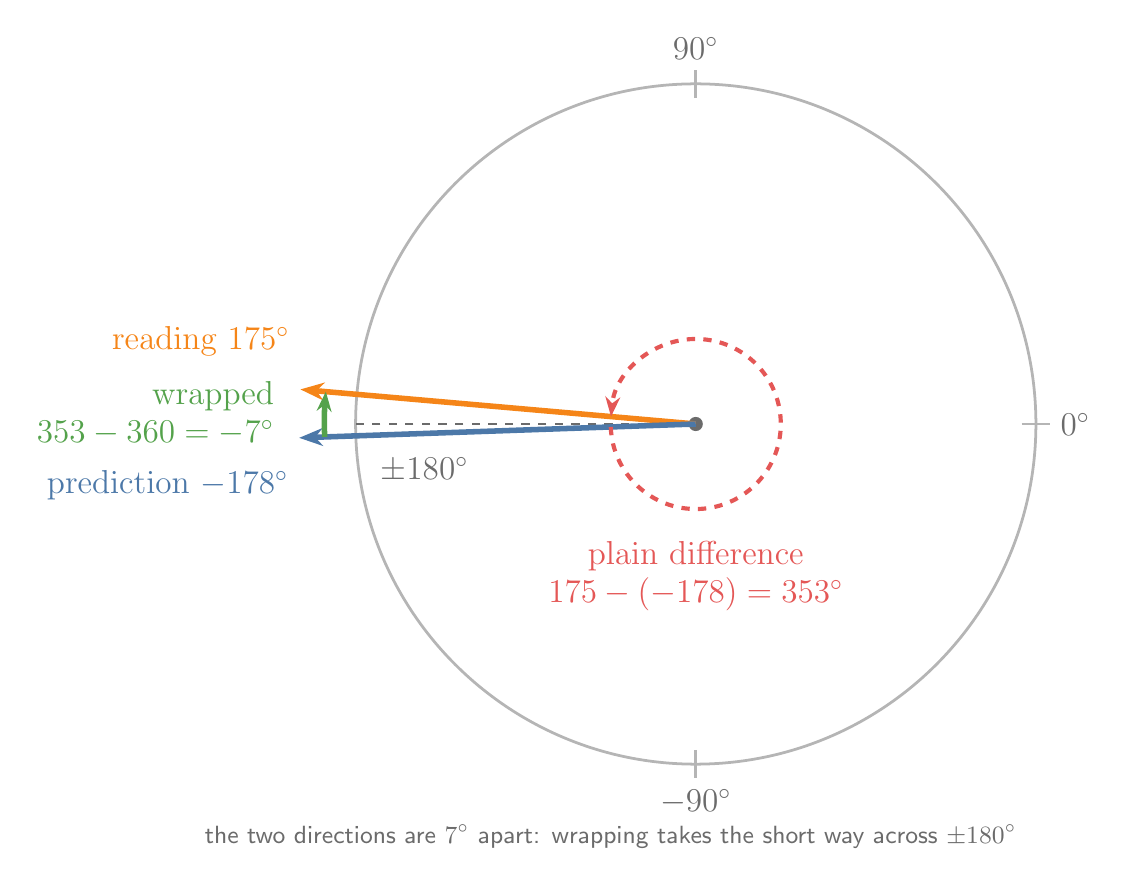
\begin{tikzpicture}[scale=1.8, every node/.append style={font=\large}]
  \draw[cgrey!50, line width=1pt] (0,0) circle (2.4);
  \foreach \a/\t/\p in {0/{$0^\circ$}/right, 90/{$90^\circ$}/above, -90/{$-90^\circ$}/below}
    \draw[cgrey!50, line width=1pt] (\a:2.3) -- (\a:2.5) node[cgrey, \p] {\t};
  \draw[cgrey, dashed, line width=1pt] (0,0) -- (180:2.4);
  \node[cgrey, anchor=north west, yshift=-8pt] at (180:2.3) {$\pm 180^\circ$};
  \fill[cgrey] (0,0) circle (0.05);
  % the two directions
  \draw[corange, line width=2pt, -{Stealth[length=3mm]}] (0,0) -- (175:2.8);
  \node[corange, anchor=south east, yshift=8pt] at (175:2.8) {reading $175^\circ$};
  \draw[cblue, line width=2pt, -{Stealth[length=3mm]}] (0,0) -- (-178:2.8);
  \node[cblue, anchor=north east, yshift=-8pt] at (-178:2.8) {prediction $-178^\circ$};
  % plain difference: from the prediction, counter-clockwise all the way round to the reading
  \draw[cred, line width=1.5pt, dashed, -{Stealth[length=2.5mm]}] (-178:0.6) arc (-178:175:0.6);
  \node[cred, anchor=north, align=center] at (0,-0.75) {plain difference\\$175 - (-178) = 353^\circ$};
  % wrapped difference: from the prediction, clockwise across the +-180 line to the reading
  \draw[cgreen, line width=2pt, -{Stealth[length=2.5mm]}] (182:2.62) arc (182:175:2.62);
  \node[cgreen, anchor=east, align=right] at (178.5:2.9) {wrapped\\$353 - 360 = -7^\circ$};
  \node[note, anchor=north] at (-0.6,-2.75) {the two directions are $7^\circ$ apart: wrapping takes the short way across $\pm 180^\circ$};
\end{tikzpicture}
\end{document}
